\documentclass[a4paper,12pt,oneside]{book}

%-------------------------------Start of the Preable------------------------------------------------
\usepackage[english]{babel}
\usepackage{blindtext}
\usepackage{color,soul}
%packagr for hyperlinks
\usepackage{hyperref}
\hypersetup{
    colorlinks=true,
    linkcolor=blue,
    filecolor=magenta,      
    urlcolor=cyan,
}

\urlstyle{same}
%use of package fancy header
\usepackage{fancyhdr}
\setlength\headheight{26pt}
\fancyhf{}
%\rhead{
\includegraphics[width=1cm]{logo}}
\lhead{\rightmark}
\rhead{
\includegraphics[width=1cm]{logo}}
\fancyfoot[RE, RO]{\thepage}
\fancyfoot[CE, CO]{\href{http://www.e-yantra.org}{www.e-yantra.org}}

\pagestyle{fancy}

%use of package for section title formatting
\usepackage{titlesec}
\titleformat{\chapter}
  {\Large\bfseries} % format
  {}                % label
  {0pt}             % sep
  {\huge}           % before-code
 
%use of package tcolorbox for colorful textbox
\usepackage[most]{tcolorbox}
\tcbset{colback=cyan!5!white,colframe=cyan!75!black,title = flush center}

\newtcolorbox{mybox}[1]{colback=cyan!5!white,
colframe=cyan!75!black,fonttitle=\bfseries,
title=\textbf{\Large{#1}}}

%use of package marginnote for notes in margin
\usepackage{marginnote}

%use of packgage watermark for pages
%\usepackage{draftwatermark}
%\SetWatermarkText{
\includegraphics{logo}}
\usepackage[scale=2,opacity=0.05,angle=0]{background}
\backgroundsetup{
contents={
\includegraphics{logo}}
}

%use of newcommand for keywords color
\usepackage{xcolor}
\newcommand{\keyword}[1]{\textcolor{red}{\textbf{#1}}}

%package for inserting pictures
\usepackage{graphicx}

%package for highlighting
\usepackage{color,soul}

%new command for table
\newcommand{\head}[1]{\textnormal{\textbf{#1}}}


%----------------------End of the Preamble---------------------------------------


\begin{document}

%---------------------Title Page------------------------------------------------
\begin{titlepage}
\raggedright
{\Large eYSIP2017\\[1cm]}
{\Huge\scshape  Navigation In Indoor  Environment Using AR Drone 2 \\[.1in]}
\vfill

{\large \hspace{3in} Team Members: \\}
\begin{flushright}
{\large Gorantla Balaji \\}
{\large Ridhwan Luthra \\} 
\end{flushright}
{\large \hspace{3.6in} Mentors: \\}
\begin{flushright}
{\large Simranjeet \\}
{\large Vamshi \\}
\vspace{5mm}
{\large Duration of Internship: $ 22/05/2017-07/07/2017 $ \\}
\end{flushright}
\vspace{5mm}
{\itshape 2017, e-Yantra Publication}
\end{titlepage}
%-------------------------------------------------------------------------------

\tableofcontents


\chapter[Abstract]{Abstract}
Drone applicability is not only limited to the outdoor applications (package delivery, surveillance, target tracking) drones can also be useful in indoor environments for manufacturing/service (e.g. hospitals, greenhouses, production companies and nuclear power plant). \\
\hspace*{0.2in} An indoor navigation system is a system that provides navigation within buildings. An indoor navigation system is a system that provides navigation within buildings. The typical GPS that we use cannot provide accurate navigation within a building and for application purpose the hardware parts we use should be of less expensive that is where we tried to avoid expensive sensors like Lidar, 3D cameras, motion capture cameras, etc., 

\section{Completion status}
Navigated the drone from one point to another point in 3D space avoiding obstacles using the given map of the environment in simulation and replicated the navigation in real world scenario successfully.


\chapter{Hardware parts}

 \section{ List of hardware} 
  \begin{itemize}
  \item 1. Parrot AR Drone 2.0 
  \item  2. ArUco markers
  \end{itemize} 
 
  \section{Detail of each hardware} 
  \begin{itemize}
  \item Here is the 
  \href{http://www.robotappstore.com/Files/KB/ARDrone/ARDrone_SDK_1_7_Developer_Guide.pdf}{AR Drone Developer guide} 
 for better understanding about AR Drone 2.0.\\\
 \begin{center}
 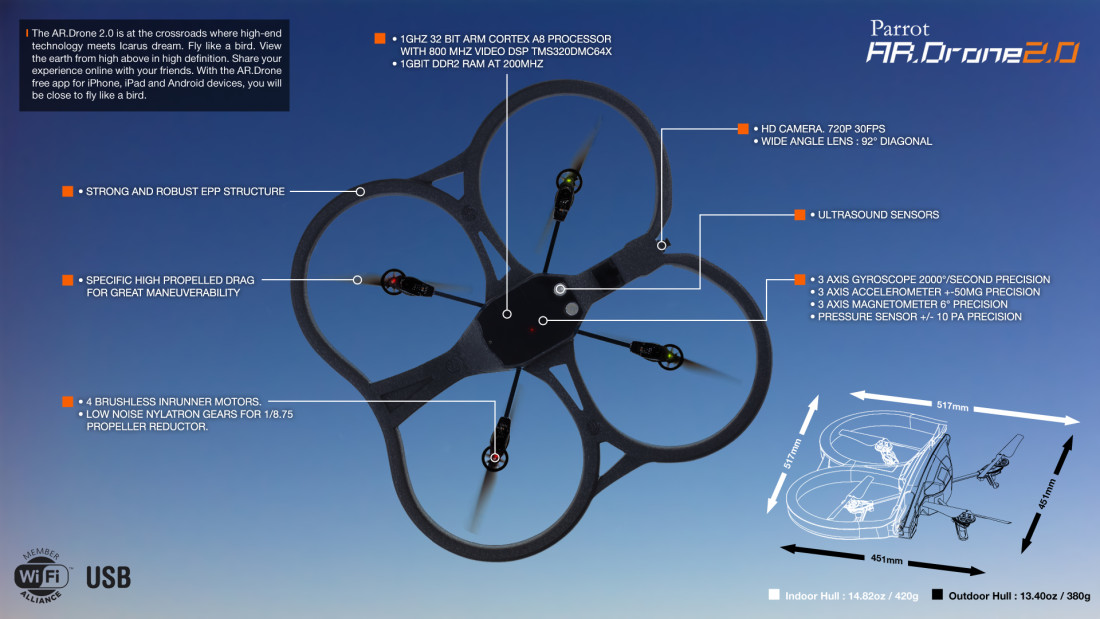
\includegraphics[scale=0.3]{drone_specs}\\
 Specification of AR Drone 2.0\\\
 \end{center}
 
  \item Here is the \href{http://docs.opencv.org/3.1.0/d5/dae/tutorial_aruco_detection.html}{ArUco marker guide} for the better understanding of creation of markers, marker detection, pose estimation using markers.
  
    \end{itemize}   

\pagebreak
\chapter[Software used]{Software used}

  \section{List of softwares used}  
  We used many packages in this project to navigate drone from one point to another. Namely -
\begin{itemize}
\item ardrone\_autonomy
\item drone\_application
\item aruco\_mapping
\item marker\_pose\_detection
\item tum\_simulator
\item MoveIt!
\end{itemize}
  \section{Details of software}  
 \begin{itemize}
 \item  \href{http://wiki.ros.org/ardrone_autonomy}{ardone\_autonomy} : This is the driver for AR drone and is necessary to communicate with the drone in simulation and in the physical world.

  
 \item  \href{http://wiki.coins-lab.org/index.php?title=Simulation_of_AR_Parrot_2}{drone\_application} : This is the package we have created for the autonomous navigation of the ardrone 2.0. 

 \item  \href{http://wiki.ros.org/aruco_mapping}{aruco\_mapping} : This package allows user to create a map of Aruco markers in 2D or 3D space and estimate full 6 DOF pose of the camera. Using Markers to estimate full 6 DOF position only by means of single calibrated camera is well known approach. This package leverages basic aruco\_ros functionality and provides tools to create a map of detected markers in 2D/3D space. 


 \item  \href{https://github.com/durovsky/marker_pose_detection}{marker\_pose\_detection} : This node publishes a visualization\_msgs/Marker on the /Estimated\_marker topic. You can Subscribe to this topic to get your location and orientation with respect to the ArUco marker.
 
 \item  \href{http://wiki.ros.org/tum_simulator}{tum\_simulator} : This package contains the implementation of a gazebo simulator for the Ardrone 2.0.

 
 
 \item   \href{ https://www.wilselby.com/research/ros-integration/3d-mapping-navigation/}{MoveIt!} : MoveIt! is state of the art software for mobile manipulation, incorporating the latest advances in motion planning, manipulation, 3D perception, kinematics, control and navigation.

 \end{itemize}

 
  \section{Installation steps}
  \hspace*{0.3in} Although ROS has been made to work on a wide variety of systems, we are using Ubuntu 14.04, a popular and relatively user-friendly Linux distribution.\\
  \hspace*{1in} This tutorial assumes that you are familiar with Linux, Python, and ROS. Also that you have already created a workspace(named catkin\_ws, if you are using a different name please change this.) and are using catkin built system. This tutorial is built for ubuntu 14.04 and ROS Indigo. \\ Ubuntu Linux can be downloaded freely from \href{http://ubuntu.com}{ubuntu}. \\
  Go through the instructions to install \href{http://wiki.ros.org/indigo/Installation/Ubuntu}{ROS Indigo}\\\
  
\begin{itemize}
\item Individual Package: You can also install a specific ROS package (replace underscores with dashes of the package name):\\\\
 \hl {sudo apt-get install ros-indigo-PACKAGE}\\\\
 To find available packages, use:\\
 \hl {apt-cache search ros-indigo}\\\\
\end{itemize}
  
If you want to install the entire functionality, you can go through the  \href{https://github.com/eYSIP-2017/eYSIP-2017_Navigation-in-Indoor-Environments-using-drone/blob/master/install_scripts/complete_install.sh}{complete\_install\_script}  
   


\pagebreak

\chapter[Approach]{Approach}
\section{Project Flow}
Here is a complete flow of our project to make it work successfully.\\
\begin{itemize}
\item Firstly, Installed ROS and necessary pacakages like ardrone\_autonomy, tum\_simulator for simulation and read the specifications of AR drone and got familierized with AR Drone 2.0.

\item Understood the concept of PID Controller and Aruco markers and used them to align the drone to the marker using the camera feed from the quadrotor in simulation and in real.

\item Worked on octomap server and generated 3D environment using turtlebot and octomap with a 3D map file. 

\item Installed Rviz and spawned the quadrotor model, 3D map in Rviz using simulator and also in real.

\item Made a literature review about the autonomous navigation.

\item Worked on aruco\_mapping package to detect the markers for localisation i.e. getting the pose of a drone from the marker.

\item Autonomously navigated the drone frome one waypoint to another by using aruco markers and odometry readings.  

\item Generated a map with the world in accordance to the objects in a room.

\item Using aruco markers for localisation, the map of the room for path planning and PID controller navigated the drone autonomously from one waypoint to another avoiding the obstacles in real world.

\end{itemize}

\chapter[Software and Code]{Software and Code}
\section{Repository}
Here is our \href{https://github.com/eYSIP-2017/eYSIP-2017_Navigation-in-Indoor-Environments-using-drone/tree/master/scripts}{Github link} for the repository of code\\\

\section{Scripts}
Brief explanation of various parts of code : \\\
\begin{itemize}
\item \href{https://github.com/eYSIP-2017/eYSIP-2017_Navigation-in-Indoor-Environments-using-drone/blob/master/scripts/ardrone_teleop_key.py}{ardrone\_teleop\_key.py} : \\
Handle Control of drone using keyboard.\\\

\item \href{https://github.com/eYSIP-2017/eYSIP-2017_Navigation-in-Indoor-Environments-using-drone/blob/master/scripts/pose.py}{pose.py} :\\
Class for pose storage.\\\

\item \href{https://github.com/eYSIP-2017/eYSIP-2017_Navigation-in-Indoor-Environments-using-drone/blob/master/scripts/localisation.py}{localisation.py} :\\
Handle usage of EKF.\\\

\item \href{https://github.com/eYSIP-2017/eYSIP-2017_Navigation-in-Indoor-Environments-using-drone/blob/master/scripts/kalman_filter.py}{kalman\_filter.py} :\\
Implimenation of Extended Kalman Filter.\\\

\item \href{https://github.com/eYSIP-2017/eYSIP-2017\_Navigation-in-Indoor-Environments-using-drone/blob/master/scripts/move\_to\_waypoint.py}{move\_to\_waypoint.py} :\\
Get drone to follow generated Trajectory.\\\

\item \href{https://github.com/eYSIP-2017/eYSIP-2017\_Navigation-in-Indoor-Environments-using-drone/blob/master/scripts/move\_to\_waypoint.py}{follow\_trajectory.py} :\\
Extract, generate and send trajectory for excecution.\\\

\item \href{https://github.com/eYSIP-2017/eYSIP-2017_Navigation-in-Indoor-Environments-using-drone/blob/master/scripts/pid.py}{pid.py} :\\
Generic PID implimentation.\\\

\item \href{https://github.com/eYSIP-2017/eYSIP-2017_Navigation-in-Indoor-Environments-using-drone/blob/master/scripts/transform_handler.py}{transform\_handler.py} :\\
Generate transform between drone's odom and aruco's world.\\\

\end{itemize}

\pagebreak

\chapter[Use and Demo]{Use and Demo}
\section{How it works}
\begin{center}
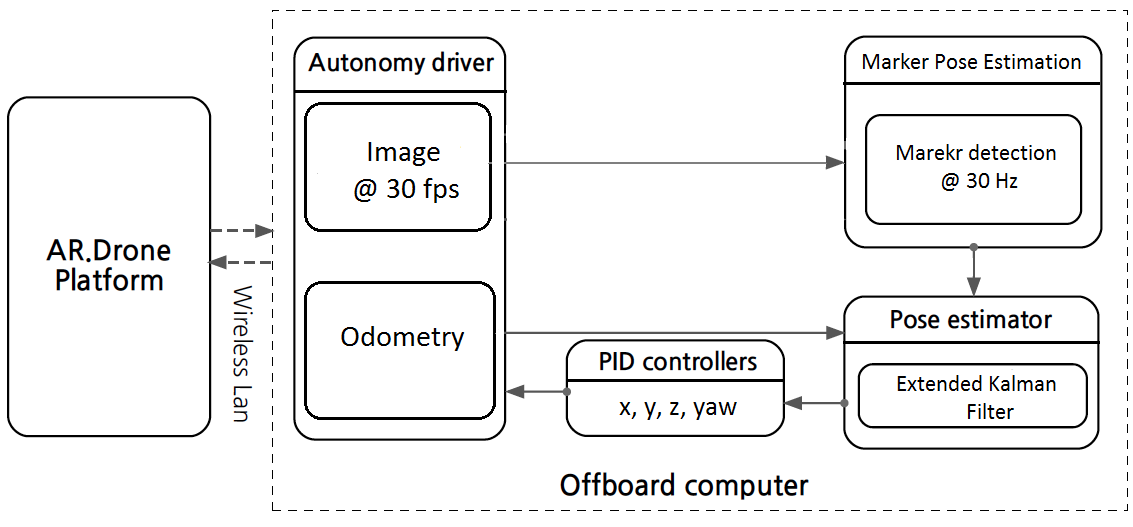
\includegraphics[scale=0.55]{pid_ardrone}\\\
\end{center}

 
\section{Instruction for demonstrations}
\begin{itemize}
\item Here is a demonstartion viedo of 
\href{https://www.youtube.com/watch?v=W7t_BQyy5vk&index=13&list=PLz8Xi5I9bhzKuFfcQxWvMm9sVCR5Wng90}{Emulating AR drone in Rviz} and follow \href{https://github.com/eYSIP-2017/eYSIP-2017_Navigation-in-Indoor-Environments-using-drone/wiki/Emulating-AR-drone-2-in-Rviz}{instructions} to emulate the AR Drone in Rviz

\item Here is a demonstartion viedo to 
\href{https://www.youtube.com/watch?v=Q2GwBIR4_pk&list=PLz8Xi5I9bhzKuFfcQxWvMm9sVCR5Wng90&index=14}{Align AR Drone 2.0 to ArUco marker} and follow \href{https://github.com/eYSIP-2017/eYSIP-2017_Navigation-in-Indoor-Environments-using-drone/wiki/Aligning-with-aruco-marker}{instructions} to align the drone with aruco marker.


\item Here is a demonstartion viedo of 
\href{https://www.youtube.com/watch?v=UVOoqWIJwnI&list=PLz8Xi5I9bhzKuFfcQxWvMm9sVCR5Wng90&index=15}{whycon marker follower ardrone in real world} and follow \href{https://github.com/eYSIP-2017/eYSIP-2017_Navigation-in-Indoor-Environments-using-drone/wiki/Aligning-with-whycon-marker}{instructions} to align the drone with whycon marker.

\item Here is a demonstartion viedo of 
\href{https://www.youtube.com/watch?v=8vy9cVHUimo&index=16&list=PLz8Xi5I9bhzKuFfcQxWvMm9sVCR5Wng90}{real world navigation of ardrone using moveit waypoints} and follow the instructions provided in video to move the drone using waypoints generated by moveit!.

\end{itemize}

\chapter[Future Work]{Future Work}
Our future works to improve our project are:\\
\begin{itemize}
\item Using sensor fusion to get reliable location.
\item Applying more robust control systems to handle the dynamics of the quadcopter.
\item Generate minimum snap trajectories for the quadrotor.
\item Handle dynamic changes in the environment.
\end{itemize}

\pagebreak

\chapter[Bug report and Challenges]{Bug report and Challenges}


Failures and challenges faced during project:\\
\begin{itemize}
\item moveit
\begin{itemize}
\item moveit is not meant for drones so adapting moveit to work with drones was a challenge.
\item We spent a week to get the entire functionality of moveit adapted for drones.
\item Finally, we used the motion planning from moveit and built our own controller to move the drone.
\end{itemize}

\item Aruco mapping
\begin{itemize}
\item Detection of markers in the aruco mapping package is not reliable when the drone is moving rapidly.
\item Applying PID became and issue as PID needs a derivative and in order for us to find the derivative the function must be continuous. We do not get a continuous function from aruco mapping and hence the edge cases needed to be handled.
\end{itemize}

\item Localisation
\begin{itemize}
\item Using dead reckoning is not an option as the odometry is not at all reliable.
\item The best solution is to apply EKF to fuse the data coming from various sensors like the aruco markers and odometry.
\item This functionality is not fully tested.
\end{itemize}

\end{itemize}


\begin{thebibliography}{li}
\bibitem{navigation}
Boaz Ben Moshe, Nir Shvalb, Junathan Baadani, Itay Nagar and Harel Levy:
{\em Indoor Positioning and Navigation for micro UAV Drones},
2012.

\bibitem{slam}
Nick Dijikshoorn:
{\em Simultaneous Localization and maping with AR Drone},
July 14,2012.

\bibitem{Motion Planning}
Anirudha Majumdar and Russ Tedrake:
{\em Funnel Libraries for Real-Time Robust Feedback Motion Planning},
May 2, 2017

\bibitem{planning}
Robin Deits and Russ Tedrake:
{\em Efficient Mixed-Integer Planning for UAVs in Cluttered Environments},

\bibitem{indoor slam}
Sergio García, M. Elena López, Rafael Barea, Luis M. Bergasa, Alejandro Gómez and Eduardo J. Molinos:
{\em Indoor SLAM for Micro Aerial Vehicles Controlusing Monocular Camera and Sensor Fusion},
2016

\bibitem{localization system}
Toma ́s Krajn ́ ˇ ık, Mat ́ıas Nitsche, Jan Faigl,
Petr Vanekˇ, Martin Saska, Libor Preu ˇ cil ˇ,Tom Duckett, Marta Mejail:
{\em A Practical Multirobot Localization System},
6 August, 2013

\bibitem{Planning and control}
Benoit Landry:
{\em Planning and Control for Quadrotor Flight through Cluttered Environments},
June, 2015

\bibitem{Planning and control}
Daniel Warren Mellinger:
{\em Trajectory Generation and Control for Quadrotors},
1 January, 2012

\end{thebibliography}


\end{document}

